\section{Extensions of the Common Quantum Algorithmic Toolbox} \label{extensions_of_the_common_quantum_algorithmic_toolbox}

The HHL algorithm requires the reader to have a rather large amount of preliminary knowledge. We shall introduce a set of common tools and their current state of the art, in the same sense as Barak \cite[p. 415]{Barak2007} referred to the \emph{quantum algorithmic toolbox}. Let \(n \in \mathbb{N}_{\geq 1}\) throughout this section. Recall some the common gates, that current books \cite{Homeister2018, Nielsen2010,Scherer2019} on quantum computer science using the unitary gate model of quantum computation present:
\begin{align}
    E_N \coloneqq (\delta_{ij})_{i, j \in N \times N} \qquad \qft_N \coloneqq \left(\omega_N^{(i-1)(j-1)}\right)_{i, j \in N \times N} \qquad H \coloneqq \frac{1}{\sqrt{2}} \begin{pmatrix}
        1 & 1\\
        1 & -1
    \end{pmatrix} \qquad \notgate \coloneqq \begin{pmatrix}
        0 & 1\\
        1 & 0
    \end{pmatrix}
\end{align}
Here is \(N \coloneqq 2^n\). Recall, that \emph{classical functions} can be efficiently simulated using a unitary of form \(\ket{x}\ket{y} \mapsto \ket{x}\ket{y \oplus f(x)}\) for a function \(f\colon \mathbb{F}_2^m \to \mathbb{F}_2^n\) with \(m \in \mathbb{N}_{\geq 1}\). Recall the concept of \emph{entangled states} from \cite[p. 95-96]{Nielsen2010}.

\begin{remark}
    When we present a quantum algorithm using an algorithm description, we normally write register tensor product terms, for instance \(\ket{\mu} \ket{\nu} = \ket{\mu} \otimes \ket{\nu}\), where \(\ket{\mu}\) and \(\ket{\nu}\) are some quantum states. Our steps can lead to an entanglement of the registers, deeming this notation to be false statements, but we shall ignore that for convenience. One may imagine a step as a application of a single large unitary, that affects all states involved.
\end{remark}

\subsection{Auxiliary Gates \draftcommentgreen{DONE}}

\paragraph*{Swapping Qubits} \phantom{}\\\phantom{}

When designing a quantum algorithm, one often needs to append auxiliary qubits for other calculations. It is often not clear, whether we can discard the auxiliary qubits afterwards. One necessary requirement for that is, that our current working state is not entangled with the auxiliary state. We call the process of preparing an auxiliary state for removal \emph{uncomputing}. The following gate assists us in that task:

\begin{definition} \label{swap_gate}
    The unitary \(\swapgate\)-gate is defined by:
    \begin{align}
        \swapgate\colon \mathbb{C}^2 \to \mathbb{C}^2, \ket{x}\ket{y} \mapsto \begin{pmatrix*}
            1 & 0 & 0 & 0\\
            0 & 0 & 1 & 0\\
            0 & 1 & 0 & 0\\
            0 & 0 & 0 & 1
        \end{pmatrix*} \ket{x}\ket{y} = \ket{y}\ket{x}
    \end{align}
\end{definition}

One may quickly observe the unitarity and correctness. By definition, the gate acts on constantly many qubits and is thus local and efficiently implementable. Successive uses of this gate allow us to uncompute multiple qubits.

\paragraph*{Rotating Qubits} \phantom{}\\\phantom{}

We present lemma 4 at \cite[p. 25]{Dervovic2018}, with which we now introduce a quantum gate for the so-called \emph{controlled rotation} of a qubit. We can imagine that as rotating the unit vector \(\ket{0}\) by some angle in the Gaussian plane, see \Cref{cr_illustration}. The mentioned paper cites this theorem for a fixed angle, but it is clear from the proof, that this can be generalized for every \(d\)-bit represented real number, \(d \in \mathbb{N}_{\geq 1}\).

We will now use our notations for floating-point-values. In case of a format like IEEE-754, the proof of the efficient implementability of the following theorem may be a bit, perhaps in form of quite a few more qubits, harder\footnote{Including special cases like infinity or NaN, of course.}.
\begin{lemma}[Controlled Rotation] \label{controlled_rotation}
    For a fixed \(d \in \mathbb{N}_{\geq 1}\), there is an with \(\onot(d)\) local gates efficiently implementable unitary that achieves for \(d\)-bit representations of angles \(\theta\):
    \begin{align}
        \controrot_d\colon \mathbb{C}^{2^{d+1}} \to \mathbb{C}^{2^{d+1}}, \ket{\theta}\ket{0} \mapsto \ket{\theta}(\cos(\theta_{\mathcal{F}})\ket{0}+\sin(\theta_{\mathcal{F}})\ket{1})
    \end{align}
    We call it the gate for \emph{controlled rotations}.
\end{lemma}
\begin{proof}
    We give a detailled version of the proof in the paper of Dervovic et. al.. Note that there is one slight subtilty: The unitary that is given in the paper is not fully correct. In the unitary, we must denote the real number, that is represented by the finite-bit representation. Let
    \begin{align}
        \controrot_d \coloneqq \sum_{\theta \in \mathbb{F}_2^d} \ket{\theta}\bra{\theta} \otimes \exp(-i\theta_{\mathcal{F}}\sigma_y) = \begin{pmatrix}
            e^{-i \cdot 0_{\mathcal{F}} \cdot \sigma_y} & 0 & \hdots & 0\\
            0 & e^{-i \cdot 1_{\mathcal{F}} \cdot \sigma_y} & \hdots & 0\\
            \vdots & \vdots & \ddots & \vdots\\
            0 & 0 & \hdots & e^{-i \cdot (2^d-1)_{\mathcal{F}} \cdot \sigma_y}
        \end{pmatrix}
    \end{align}
    Note that, in the definition, \(\theta\) is a bitvector and interpreted as its associated natural number. For any \(\ket{\theta} \in \mathbb{F}_2^d\), it holds that:
    \begin{align}
        \controrot_d\ket{\theta}\ket{0} = \ket{\theta}\exp(-i\theta_{\mathcal{F}}\sigma_y)\ket{0} = \ket{\theta}\exp\begin{pmatrix}
            0 & -\theta_{\mathcal{F}}\\
            \theta_{\mathcal{F}} & 0
        \end{pmatrix}\ket{0} \overset{\ref{helper_calc_3_1}}{=} \ket{\theta}(\cos(\theta_{\mathcal{F}})\ket{0}+\sin(\theta_{\mathcal{F}})\ket{1})
    \end{align}
    \begin{enumerate}[label=(\arabic*)]
        \item \label{helper_calc_3_1} We use \Cref{definition_matrix_exponential_function} and \Cref{sine_and_cosine_taylor_series} to obtain
        \begin{align}
            &\exp\begin{pmatrix}
                0 & -\theta_{\mathcal{F}}\\
                \theta_{\mathcal{F}} & 0
            \end{pmatrix} = \sum_{k=0}^\infty \frac{1}{k!} \begin{pmatrix}
                0 & -\theta_{\mathcal{F}}\\
                \theta_{\mathcal{F}} & 0
            \end{pmatrix}^k\\
            =& \sum_{k=0}^\infty \frac{1}{(2k)!} \begin{pmatrix}
                0 & -\theta_{\mathcal{F}}\\
                \theta_{\mathcal{F}} & 0
            \end{pmatrix}^{2k} + \sum_{k=0}^\infty \frac{1}{(2k+1)!} \begin{pmatrix}
                0 & -\theta_{\mathcal{F}}\\
                \theta_{\mathcal{F}} & 0
            \end{pmatrix}^{2k+1}\\
            =& \sum_{k=0}^\infty \frac{1}{(2k)!} \begin{pmatrix}
                (-1)^k\theta_{\mathcal{F}}^{2k} & 0\\
                0 & (-1)^k\theta_{\mathcal{F}}^{2k}
            \end{pmatrix} + \sum_{k=0}^\infty \frac{1}{(2k+1)!} \begin{pmatrix}
                0 & -(-1)^k\theta_{\mathcal{F}}^{2k+1}\\
                (-1)^k\theta_{\mathcal{F}}^{2k+1} & 0
            \end{pmatrix}\\
            =& \begin{pmatrix}
                \cos(\theta_{\mathcal{F}}) & -\sin(\theta_{\mathcal{F}})\\
                \sin(\theta_{\mathcal{F}}) &  \cos(\theta_{\mathcal{F}})
            \end{pmatrix}
        \end{align}
    \end{enumerate}
    To observe the claimed runtime, we give a high level description of a possible implementation. For any basis state \(\ket{\theta}\), we may define a local unitary rotation, as in \Cref*{example_unitary_rotation}, for each bit of the representation, successively rotating the ancilla bit by some degrees each time. This does not violate the correctness, as the rotation map in the plane is linear. It is clear, that we only require \(d\) such gates and thus \(\onot(d)\) many local unitary gates.
\end{proof}

\begin{figure}[!hbtp]
    \centering
    \begin{tikzpicture}[>=stealth, semithick]
        \node at (0, 0) {\(\ket{\theta} \in \mathbb{C}^{2^d}\)};
        \node at (1, 0) {\(\leadsto\)};
        \coordinate (a) at (3.5, 0);
        \coordinate (b) at (5, 0);
        \coordinate (c) at (3.5-0.7071*1.5, 0.7071*1.5);
        \draw[->] (1.5, 0) -- (5.5, 0) node[right] {\(\ket{0}\)};
        \draw[->] (3.5, -2) -- (3.5, 2) node[above] {\(\ket{1}\)};
        \draw pic[->, draw=black, angle eccentricity=0.5, angle radius=0.75cm, fill=white]
        {angle=b--a--c};
        \draw[->] (a) -- (b);
        \draw[->] (a) -- (c);
        \node at (3.75, 0.3) {\(\theta_{\mathcal{F}}\)};
    \end{tikzpicture}
    \caption{Unit vector rotations, controlled by qubit registers. Here for \(\theta_{\mathcal{F}} = 3\pi/4\).}
    \label{cr_illustration}
\end{figure}

\subsection{Quantum State Generation based on Efficiently Integrable Probability Distributions \draftcommentgreen{DONE}} \label{quantum_state_generation_based_on_efficiently_integrable_probability_distributions}

\begin{problem}{(Quantum State Generation)}
    Suppose one is given an initial state \(\ket{\psi} \in \mathbb{C}^N\) and another state \(\sum_{\tau = 0}^{T-1} \alpha_\tau \ket{\tau}\). Give an efficient quantum algorithm, that performs the map \(\ket{\psi} \mapsto \sum_{\tau = 0}^{T-1} \alpha_\tau \ket{\tau}\).
\end{problem}

This problem has been studied extensively. Approaches include the most direct method of successive rotation of the initial state into the target state \cite{Kaye2004, Mottonen2004}, which in both algorithms requires an exponential runtime. Aharonov et al. \cite{Aharonov2003} have studied the problem in the framework of \emph{Adiabatic Quantum Computation}, a different framework for quantum algorithms using the so-called \emph{Adiabatic theorem} from QM \cite[p. 426 ff.]{Griffiths2018}. There are no hardness results yet, to my knowledge. There is a simple combinatorial argument, that speaks against the existence of such circuits for any state, if we want to use a predefined set of finitely many gates \cite[pp. 198-200]{Nielsen2010}. One could say that no finite system of gates is complete wrt. efficient quantum state generation. Consider the following theorem with contained proof.

\begin{theorem}
    Let \(f, g \in \mathbb{N}_{\geq 1}\). Using \(g\) many efficient \(n\)-qubit-gates, each acting on at most \(f\) qubits, one can generate at most \(\binom{n}{f}^gm \in \onot(n^{fgm})\) states using \(m\) gates from \(\ket{0}\).
\end{theorem}

We shall discuss a classical paper from 2002 by the researchers Grover and Rudolph \cite{Grover2002}. It focuses on the case, where the coefficients \(\alpha_\tau, \tau \in [0, T-1]_{\mathbb{N}}\) are given by \emph{efficiently integrable probability density functions}.

\begin{definition}
    Let \(I \subseteq \mathbb{R}\), \(I \neq \emptyset\), be compact and connected. We call a Riemann-integrable function \(f\colon I \to \mathbb{R}\) \emph{efficiently integrable}, if for any \(x_0, x_1 \in I\) with \(x_0 \leq x_1\), we can compute or at approximate \(\int_{x_0}^{x_1} f\) in polynomial time.
\end{definition}

The following theorem summarizes the result.

\begin{theorem}[Quantum State Generation using Efficiently Integrable Probability Distributions] \label{qsg_using_efficient_integrable_probability_distributions}
    Let \(x_L^{m, i} \coloneqq i/2^m, x_R^i \coloneqq (i+1)/2^m\) for any \(m \in \mathbb{N}_{\geq 1}, i \in [0, 2^m-1]_{\mathbb{N}}\). For an arbitrary quantum state \(\sum_{\tau = 0}^{T-1} \alpha_\tau \ket{\tau}\) with \(t \in \mathbb{N}_{\geq 1}, T \coloneqq 2^t\), s.t. there is a classically efficiently integrable probability density function \(p\colon [0, 1] \to [0, 1]\) with \(\alpha_\tau = \sqrt{\int_{[x_L^{t, \tau}, x_R^{t, \tau}]} p}\), there is a quantum algorithm, that solves the state generation problem \(\ket{0} \mapsto \sum_{\tau = 0}^{T-1} \alpha_\tau \ket{\tau}\) up to an arbitrary precision using some number of helper qubits, whilst being polynomial in \(t\).
\end{theorem}

\begin{proof}
    The squared amplitude magnitudes of our goal quantum state \(\{|\alpha_\tau|^2 \mid \tau \in [0, T-1]_{\mathbb{N}}\}\) form a discrete probabiliy distribution. The probability space corresponds to the tuple \(([0, T-1]_{\mathbb{N}}, \text{Pr})\) with \(\text{Pr}\colon [0, T-1]_{\mathbb{N}} \to [0, 1], \tau \mapsto |\alpha_{\tau}|^2\). We perform \(t\) successive and even divisions of the interval \([0, 1]\) and associate with each of these \(t+1\) intervals a probability distribution \(\{p_i^m \mid i \in [0, 2^m-1]_{\mathbb{N}}\}\), where \(m \in [0, t]_{\mathbb{N}}\) and:
    \begin{align}
        p_i^m \coloneqq \sum_{\tau = 2^{t-m}i}^{2^{t-m}(i+1)-1} p^t_\tau
    \end{align}
    Note that \(p_0^0 = 1\), \(p_\tau^t = |\alpha_\tau|^2\) by construction and especially:
    \begin{align}
        \sum_{\tau = 2^{t-m}i}^{2^{t-m}(i+1)-1} p^t_\tau = \sum_{\tau = 2^{t-m}i}^{2^{t-m}(i+1)-1} \int_{x_L^{t, \tau}}^{x_R^{t, \tau}} p = \int_{x_L^{m, i}}^{x_R^{m, i}} p
    \end{align}
    Since \(p\) is classically efficiently computable, we can use our knowledge from quantum computability theory. We can construct a set of functions \(f_m\) as follows:
    \begin{align}
        f_m \colon [0, 2^m-1]_{\mathbb{N}} \to [0, 1], i \mapsto \frac{\int_{x_L^{m, i}}^{\frac{x_L^{m, i}+x_R^{m, i}}{2}} p(x) \, dx}{\int_{x_L^{m, i}}^{x_R^{m, i}} p(x) \, dx} \overset{\ref{helper_calc_4_1}}{=} \frac{\int_{x_L^{m+1, 2i}}^{x_R^{m+1, 2i}} p(x) \, dx}{\int_{x_L^{m, i}}^{x_R^{m, i}} p(x) \, dx} = \frac{p_{2i}^{m+1}}{p_i^m}
    \end{align}
    \begin{enumerate}[label=(\arabic*)]
        \item \label{helper_calc_4_1} By definition: \((x_L^{m, i}+x_R^{m, i})/2 = (i+i+1)/2^{m+1} = x_R^{m+1, 2i}, x_L^{m, i} = 2i/2^{m+1} = x_L^{m+1, 2i}\).
    \end{enumerate}
    
    The idea is to extend some current \(m\)-qubit register, that is initialized with amplitudes from the target distribution, by one qubit each time. Wlog., we may assume \(m \geq 1\) for the indices in the following calculations. If we have not initialized any qubit register yet, we can still apply the following analogously. Assume that we have already initialized this distribution-based quantum state for \(m < t\) many qubits and are not finished, meaning that we have a register:
    \begin{align}
        \sum_{i = 0}^{2^m-1} \sqrt{\sum_{\tau = 2^{t-m}i}^{2^{t-m}(i+1)-1} p_\tau} \ket{i} = \sum_{i=0}^{2^m-1} \sqrt{p_i^m} \ket{i}
    \end{align}
    Denote the unitary:
    \begin{align}
        U_{f_m}\colon \mathbb{C}^{2^{m+d}} \to \mathbb{C}^{2^{m+d}}, \ket{x}\ket{y} \mapsto \ket{x}\ket{y \oplus \arccos(\sqrt{f_m(x)})} \eqqcolon \ket{x}\ket{y \oplus \theta_x}
    \end{align}
    Where \(d \in \mathbb{N}_{\geq 1}\) is an arbitrary amount of auxiliary qubits and the exclusive disjunction is taken bitwise. Also note that the computed \(\arccos\) and \(\sqrt{...}\) functions are approximations of the corresponding real-valued functions. We leave this part to numerical mathematicians and add an additional qubit to this register and perform the computation:
    \begin{align}
        \sum_{i=0}^{2^m-1} \sqrt{p_i^m}\ket{i}\ket{0...0}\ket{0} &\xmapsto{\parbox{2.75cm}{\centering \(U_{f_m} \times E_2\)}} \sum_{i=0}^{2^m-1}\sqrt{p_i^m}\ket{i}\ket{\theta_i}\ket{0}\\
        &\xmapsto{\parbox{2.75cm}{\centering \(E_{2^m} \times \controrot_d\)}} \sum_{i=0}^{2^m-1}\sqrt{p_i^m}\ket{i}\ket{\theta_i}(\cos(\theta_i)\ket{0}+\sin(\theta_i)\ket{1})\\
        &\xmapsto{\parbox{2.75cm}{\centering \(U_{f_m}^\dagger \times E_2\)}} \sum_{i=0}^{2^m-1}\sqrt{p_i^m}\ket{i}\ket{0}(\cos(\theta_i)\ket{0}+\sin(\theta_i)\ket{1})\\
        &\xmapsto{\parbox{2.75cm}{\centering \(E_{2^{m+d-1}} \times \swapgate\)}} \sum_{i=0}^{2^m-1}\sqrt{p_i^m}\ket{i}\ket{0}(\cos(\theta_i)\ket{0}+\sin(\theta_i)\ket{1})\ket{0}\\
        &\overset{\ref{helper_calc_1_1}}{\leadsto} \sum_{i=0}^{2^m-1}\sqrt{p_i^m}\ket{i}(\cos(\theta_i)\ket{0}+\sin(\theta_i)\ket{1})\ket{0}\\
        &= \sum_{i=0}^{2^m-1}\sqrt{p_i^m}\ket{i}\left(\sqrt{f_m(i)}\ket{0}+\sqrt{1-f_m(i)}\ket{1}\right)\ket{0}
    \end{align}
    \begin{enumerate}[label=(\arabic*)]
        \item \label{helper_calc_1_1} We perform the previous swap operation \(d-1\) additional times to push out the remaining helper bits.
    \end{enumerate}

    Since we uncomputed the helper register, it can be reused for other tasks. Although it is not obvious, the following computation shows that this corresponds to our target state.
    \begin{align}
        \sum_{i=0}^{2^m-1}\sqrt{p_i^m}\ket{i}\left(\sqrt{f_m(i)}\ket{0}+\sqrt{1-f_m(i)}\ket{1}\right) &= \sum_{i=0}^{2^m-1}\sqrt{p_i^m}\ket{i}\left(\sqrt{\frac{p_{2i}^{m+1}}{p_i^m}}\ket{0}+\sqrt{\frac{p_i^m-p_{2i}^{m+1}}{p_i^m}}\ket{1}\right)\\
        &\overset{\ref{helper_calc_2_1}}{=} \sum_{i=0}^{2^m-1}\sqrt{p_i^m}\ket{i}\left(\sqrt{\frac{p_{2i}^{m+1}}{p_i^m}}\ket{0}+\sqrt{\frac{p_{2i+1}^{m+1}}{p_i^m}}\ket{1}\right)\\
        &= \sum_{i=0}^{2^{m+1}-1}\sqrt{p_i^{m+1}}\ket{i}
    \end{align}
    \begin{enumerate}[label=(\arabic*)]
        \item \label{helper_calc_2_1} Just to be precise, we calculate this by definition. Some index play yields:
        \begin{align}
            p_i^m-p_{2i}^{m+1} &= \textstyle\sum_{\tau=2^{t-m}i}^{2^{t-m}(i+1)-1} p_\tau - \textstyle\sum_{\tau=2^{t-m-1}2i}^{2^{t-m-1}(2i+1)-1} p_\tau = \textstyle\sum_{\tau=2^{t-m}i}^{2^{t-m}i+2^{t-m}-1} p_\tau - \textstyle\sum_{\tau=2^{t-m}i}^{2^{t-m}i+2^{t-m-1}-1} p_\tau\\
            &= \textstyle\sum_{\tau=2^{t-m}i+2^{t-m-1}}^{2^{t-m}i+2^{t-m}-1} p_\tau = \textstyle\sum_{\tau=2^{t-m-1}(2i+1)}^{2^{t-m-1}(2i+2)-1} p_\tau = p_{2i+1}^{m+1}
        \end{align}
    \end{enumerate}

    Which was the desired state. So the trick here is to use the angle approximation as an angle in a rotation, but by that we introduce it as an amplitude, which gives the desired result.

    All gates are efficiently implementable. Every iteration requires polynomial time. In total, we iterate \(t\) times, concluding the claimed runtime for \(d \in \onot(1)\).
\end{proof}

\begin{remark} One may notice
    \begin{itemize}
        \item one remarkable aspect of quantum computing also shows in this proof: Each construction iteration, the superposition of states gets doubled in \(\onot(1)\) quantum runtime. This choice of the clock register coefficients is also due to the error analysis.
        \item that the requirement of efficient integrability may be relaxed by the requirement of efficient integrability over the parts of the interval divisions considered.
    \end{itemize}
\end{remark}

We restrict ourselves to the interval \([0, 1]\) in both domain and image for simplicity and the procedure, but one can think about generalizing the result by adjusting the interval division and possibly introducing special indices for subintervals starting in \(-\infty\) or ending in \(\infty\).

\begin{remark}[Discussion and Outlook]
    The proof of the above theorem from Grover and Rudolph shows, that, we can, in principle, construct any arbitrary quantum state, given the coefficients. A general, but inefficient integration can be achieved by the classical function just summing up the coefficients of the contained smallest intervals of level \(t\) in the current subinterval. Efficient schemes, such as utilizing binary trees, which may remind a computational geometrician of interval trees \cite[p. 220-226]{Berg2008}, may allow for the logarithmic lookup of these sums, but such a data structure itself will still require \(\onot(N \log(N))\) space complexity. The idea of employing tree-like structures has been studied in a PhD thesis \cite[pp. 23-27]{Dervovic2018}.
\end{remark}

\begin{figure}[!hbtp]
    \centering
    \begin{tikzpicture}[>=stealth, scale=2, semithick]
        \draw[pattern=north east lines] plot [smooth] coordinates { (0, 0) (0.5, 0.75) (0.66, 0.5) (0.75, 1) (1.0, 0.4) (1.5, 0.66) (2.0, 0.25) (2.5, 0.33) (3.0, 0.13) (3.5, 0) };
        \fill[white] (0, 0) -- (0.875, 0) -- (0.875, 1) -- (0, 1) -- cycle;
        \fill[white] (1.75, 0) -- (3.5, 0) -- (3.5, 1) -- (1.75, 1) -- cycle;
        \newcommand{\intervaldiv}[2]{
            \draw[-] (0, #1) -- (3.5, #1);
            \foreach \x in {0, 1, ..., #2} {
                \draw (3.5*\x/#2, #1-0.05) -- (3.5*\x/#2, #1+0.05);
            }
        };
        % NOTE: Rough definition due to time constraints.
        \newcommand{\intervaldivprobcap}[4]{
            \foreach \x in {0, ..., #4} {
                \node[below] at (3.5*\x/#3+3.5*1/2*1/#3, #1) {\(p^#2_\x\)};
            }
        };
        \draw[->] (0, 0) -- (0, 1) node[above, pos=1.0] {\(p(x)\)};
        \draw[->] (0, 0) -- (3.5, 0) node[below, pos=0.0] {\(0\)} node[below, pos=1.0] {\(1\)} node[right, pos=1.0] {\(x\)};
        \intervaldiv{-0.50}{1};
        \intervaldiv{-1.00}{2};
        \intervaldiv{-1.50}{4};
        \intervaldiv{-2.00}{8};
        \node at (1.75, -2.50) {\(\vdots\)};
        \intervaldiv{-3.00}{64};
        \intervaldivprobcap{-0.50}{0}{1}{0};
        \intervaldivprobcap{-1.00}{1}{2}{1};
        \intervaldivprobcap{-1.50}{2}{4}{3};
        \intervaldivprobcap{-2.00}{3}{8}{7};
        \node[right] at (3.75, -0.50) {\(m = 0, ([0, 0]_{\mathbb{N}}, i \mapsto p_i^0), \sum_{i=0}^0 p_i^0 \ket{i}\)};
        \node[right] at (3.75, -1.00) {\(m = 1, ([0, 1]_{\mathbb{N}}, i \mapsto p_i^1), \sum_{i=0}^1 p_i^1 \ket{i}\)};
        \node[right] at (3.75, -1.50) {\(m = 2, ([0, 3]_{\mathbb{N}}, i \mapsto p_i^2), \sum_{i=0}^3 p_i^2 \ket{i}\)};
        \node[right] at (3.75, -2.00) {\(m = 3, ([0, 7]_{\mathbb{N}}, i \mapsto p_i^3), \sum_{i=0}^7 p_i^3 \ket{i}\)};
        \node (1) at (-0.05, -2.50) {\(\vdots\)};
        \path[->] (-0.05, -0.50) edge[bend right=45] (-0.05, -1.00)
                  (-0.05, -1.00) edge[bend right=45] (-0.05, -1.50)
                  (-0.05, -1.50) edge[bend right=45] (-0.05, -2.00)
                  (-0.05, -2.00) edge[bend right=45] (1)
                  (1) edge[bend right=45] (-0.05, -3.00);
        \node[right] at (3.75, -3.00) {\(m = t, ([0, 2^t-1]_{\mathbb{N}}, i \mapsto p_i^t), \sum_{i=0}^{T-1} p_i^t \ket{i}\)};
        \draw plot [smooth] coordinates { (0, 0) (0.5, 0.75) (0.66, 0.5) (0.75, 1) (1.0, 0.4) (1.5, 0.66) (2.0, 0.25) (2.5, 0.33) (3.0, 0.13) (3.5, 0) };
        \draw[->, dotted] (1.3125, 0.00) -- (1.3125, -1.50);
        % Dirty approximation.
        \draw (0.875, 0) -- (0.875, 0.645);
        \draw (1.75, 0) -- (1.75, 0.46);
    \end{tikzpicture}
    \caption{Sketch for understanding the divisions. Here for \(t = 6\) and captions only in the first four divisions to avoid cluttering the sketch. The vertical axis has no markings as the image of the function \(p\) is drawn solely for illustration. On the right, the associated value of \(m\), the associated discrete probability space and the corresponding state are denoted. The arrows on the left illustrate the direction of the inductive algorithm by Grover and Harris. The part of the area under the curve of \(p\), which gives \(p_1^2\), has been highlighted.}
\end{figure}

\subsection{Quantum Mechanical Metrics \draftcommentgreen{DONE}}

\paragraph*{State Similarity} \phantom{}\\\phantom{}

Let \(\ket{\varphi}, \ket{\psi} \in \mathbb{C}^n\) be two quantum states for this part. To compare the similarity between them, one can use the introduced standard norm and define a metric by \(\norm{\ket{\varphi}-\ket{\psi}}\).

\begin{theorem}
    The tuple \((\{\ket{\psi} \in \mathbb{C}^n \mid \norm{\ket{\psi}} = 1\}, d_n)\) is a metric space, where \(d_n\) is the map
    \begin{align}
        d_n \colon \mathbb{C}^n \times \mathbb{C}^n \to \mathbb{R}_{\geq 0}, (\ket{\varphi}, \ket{\psi}) \mapsto \norm{\ket{\varphi}-\ket{\psi}}
    \end{align}
\end{theorem}

The proof can be found in \cite[p. 1-2]{Werner2018}, the definition of a metric can be found in \cite[p. 551]{Werner2018}. This theorem, to us, has semantical meaning. The complex vector norm induces a metric, meaning that we can measure the similarity between states by computing the above formula. A short rewrite yields the following theorem.

\begin{theorem} \label{state_similarity_theorem}
    It holds, that
    \begin{align}
        \norm{\ket{\varphi}-\ket{\psi}} = \sqrt{2(1-\Re(\braket{\varphi}{\psi}))}
    \end{align}
\end{theorem}

\begin{proof}
    We use the additivity of the complex standard product in both components and compute:
    \begin{align}
        \norm{\ket{\varphi}-\ket{\psi}}^2 &= \braket{\ket{\varphi}-\ket{\psi}}{\ket{\varphi}-\ket{\psi}}\\
        &= \braket{\varphi}{\varphi}-\braket{\psi}{\varphi}-\braket{\varphi}{\psi}+\braket{\psi}{\psi}\\
        &\overset{\ref{norm_rewrite_1}}{=} 2(1-\Re(\braket{\varphi}{\psi}))
    \end{align}
    \begin{enumerate}[label=(\arabic*)]
        \item \label{norm_rewrite_1} We use, that \(\norm{\ket{\varphi}}^2 = \norm{\ket{\psi}}^2 = 1\). Furthermore, we have
        \begin{align}
            \braket{\psi}{\varphi}+\braket{\varphi}{\psi} = \sum_{i=1}^n \varphi_i\psi_i^* + \sum_{i=1}^n \varphi_i^*\psi_i
        \end{align}
        However, \(\varphi_i\psi_i^* + \varphi_i^*\psi_i = 2\varphi_{i1}\psi_{i1} + 2\varphi_{i2}\psi_{i2}\). So \(\braket{\psi}{\varphi}+\braket{\varphi}{\psi} = 2\Re(\braket{\varphi}{\psi})\).
    \end{enumerate}
\end{proof}

\paragraph*{Operator Similarity} \phantom{}\\\phantom{}

Similarly to state similarity, there are norms for operators, which allow us to, for instance, analyze the error of a quantum algorithm. With \cite[p. 51]{Werner2018} in mind, we introduce the following theorem.

\begin{theorem} \label{operator_norm}
    The following map is a norm, the so-called \emph{operator norm}:
    \begin{align}
        \norm{\cdot}\colon \mathbb{C}^{n \times n} \to \mathbb{R}_{\geq 0}, A \mapsto \max_{\substack{\ket{\varphi} \in \mathbb{C}^n\\\norm{\ket{\varphi}} = 1}} \norm{A\ket{\varphi}}
    \end{align}
\end{theorem}

\begin{proof}
    Let \(S \coloneqq \{\ket{\varphi} \in \mathbb{C}^n \mid \norm{\ket{\varphi}} = 1\}\). The map is well-defined, since linear maps over \(\mathbb{C}^n\) are continuous and \(S\) is closed and bounded by definition wrt. the standard topology over \(\mathbb{C}^n\), thus by Heine-Borel \cite[p. 41]{Forster2017} compact. So the maximum always exists \cite[p. 43]{Forster2017}. To be precise, the closedness is due to one being able to span a line between a point outside of \(S\) and \(0\) and taking the distance to the point hit on \(S\) as the associated open set for the point, the boundedness, due to the fact, that \(\max\{\norm{\ket{v}}\} = 1 < 2\), so \(S \subset \{v \in \mathbb{C}^n \mid \norm{v} < 2\}\).
    
    The homogenity follows from \(\norm{(zA)\ket{\varphi}} = |z|\norm{A\ket{\varphi}}\), which carries over into the maximum. The triangle inequality also carries over from the norm of \(\mathbb{C}^n\). Lastly, the positive-definiteness is obtained by observing, that if the vectors of an arbitrary base are all mapped to zero, the linear map itself must be zero. This concludes the proof.
\end{proof}

\begin{example}
    Consider the operator given by
    \begin{align}
        A \coloneqq \begin{pmatrix}
            1 & 0\\
            i & 0
        \end{pmatrix}
    \end{align}
    Then for any \((b_1, b_2) \in \mathbb{C}^2\), \(\norm{A \begin{pmatrix}b_1 & b_2\end{pmatrix}^t}^2 = 2|b_1|^2\), so \(\norm{A} = \sqrt{2}\).
\end{example}

This norm also induces a metric, as the norm for states did.

\begin{remark}[Comparing Operators]
    To compare two operators \(U\) and \(U'\) and prove a bound for the operator distance \(\norm{U-U'}\), it suffices to bound the distance \(\norm{U\ket{\varphi}-U'\ket{\varphi}}\), with \(\ket{\varphi}\) being an arbitrary quantum state.
\end{remark}

\subsection{Qutrits \draftcommentgreen{DONE}} \label{subsection_qutrits}

Whilst qubits are the quantum equivalent of bits, \(\emph{qutrits}\) imitate the concept of a \(\emph{trit}\). Such electrical devices allow us to store three states, instead of two. In some systems, we denote them as \(0, 1, 2\) and in others in form of the \emph{balanced representation} \(-1, 0, 1\) for convenience \cite[p. 1]{Parhami_2013}. A qutrit is a member of \(\mathbb{C}^3\). We denote the canonical base as \(\{\ket{0}, \ket{1}, \ket{2}\}\) \cite[pp. 2-3]{Gokhale2019}.

We want to study three-dimensional rotations of qutrits. First, we give a lemma, which we derive from \cite[pp. 70-75]{Janich2010}.

\begin{definition}
    Let
    \begin{align}
        \times\colon \mathbb{R}^3 \times \mathbb{R}^3 \to \mathbb{R}^3, (u, v) \mapsto \begin{pmatrix}
            u_2v_3-u_3v_2\\
            u_3v_1-u_1v_3\\
            u_1v_2-u_2v_1
        \end{pmatrix}
    \end{align}
    be the so-called \emph{cross product}.
\end{definition}

\begin{lemma} \label{lemma_definition_cross_product}
    If \(\{u, v\} \subseteq \mathbb{R}^3\) is an orthonormal system, then \(\{u, v, u \times v\}\) is an orthonormal basis.
\end{lemma}

The proof can be found in the above-mentioned literature. When constructing three-dimensional unitaries, the cross product proves to be useful, as we will see in the proof of the following theorem.

\begin{theorem}[Three-Dimensional Qutrit Rotation] \label{qutrit_rotation}
    For a \(m \in \mathbb{N}_{\geq 1}\)-qubit-register with an appended qutrit and classically efficiently computable functions \(f\colon \mathbb{R} \to \mathbb{R}\), \(g\colon \mathbb{R} \to \mathbb{R}\), s.t. \(f^2+g^2 \leq 1\) and \(g^2(x) \neq 1\) for all \(x \in \mathbb{R}\), there is an efficient quantum algorithm, that achieves for any desirable precision
    \begin{align}
        \mathbb{C}^{2^m \cdot 3} \to \mathbb{C}^{2^m \cdot 3}, \ket{\lambda}\ket{0} \mapsto \ket{\lambda}(\sqrt{1-f^2(\lambda)-g^2(\lambda)}\ket{0}+f(\lambda)\ket{1}+g(\lambda)\ket{2})
    \end{align}
\end{theorem}

\begin{proof}
    We start off with a geometric argument on three-dimensional rotations. One notices, that the desired state of the qutrit is normalized, and that the amplitudes of the state vector are real. We can imagine the problem as moving the vector \(\ket{0}\) on the real unit sphere \(S^2\) into our target state, as depicted in \Cref{qutrit_rotation_figure}.
    
    We now directly explain, how to rotate the qutrit state \(\ket{0}\) into an arbitrary qutrit state of form \(\ket{\xi} \in \mathbb{R}^3\). Let \(P_{01} \coloneqq \ket{0}\bra{0} + \ket{1}\bra{1}\). \(\varphi \coloneqq \sphericalangle(\ket{0}, P_{01}\ket{\xi}), \psi \coloneqq \sphericalangle(P_{01}\ket{\xi}, \ket{\xi})\). Let \((\varphi, \psi) = (0, \pi/2)\), if \(\ket{\xi}_3 = 1\) and \((\varphi, \psi) = (0, 3\pi/2)\) for \(\ket{\xi}_3 = -1\). Note, that \(P_{01}\) performs the projection onto the plane spanned by \(\{\ket{0}, \ket{1}\}\). First, we rotate \(\ket{0}\) along the plane spanned by \(\{\ket{0}, \ket{1}\}\) by angle \(\varphi\). Then, we rotate the resulting vector \(P_{01}\ket{\xi}\) by the angle \(\psi\) along the plane spanned by \(\{P_{01}\ket{\xi}, \ket{2}\}\) into \(\ket{\xi}\).
    
    The two-dimensional standard rotation matrix, as seen in \Cref{controlled_rotation}, is for some \(\theta \in (-\pi, \pi]\)
    \begin{align}
        \begin{pmatrix}
            \cos(\theta) & -\sin(\theta)\\
            \sin(\theta) &  \cos(\theta)
        \end{pmatrix}
    \end{align}
    In three dimensions, we can always fix one coordinate and look at the cartesian coordinate system, that is spanned, when the canonical unit vector of the fixed coordinate points upwards and the others point downwards. Especially, \(\ket{2}\) is to the right of \(\ket{0}\). Otherwise, \(\ket{0}\) is right of \(\ket{1}\) and \(\ket{1}\) is right of \(\ket{2}\). To rotate in these induced planes, we look at the rotation matrices of form
    \begin{align}
        R_x(\theta) \coloneqq \begin{pmatrix}
                       1 &             0 &             0\\
                       0 &  \cos(\theta) & -\sin(\theta)\\
                       0 &  \sin(\theta) &  \cos(\theta)
        \end{pmatrix},
        R_y(\theta) \coloneqq \begin{pmatrix}
            -\sin(\theta) &             0 & \cos(\theta)\\
                        0 &             1 &            0\\
             \cos(\theta) &             0 & \sin(\theta)
        \end{pmatrix},
        R_z(\theta) \coloneqq \begin{pmatrix}
            \cos(\theta) & -\sin(\theta) & 0\\
            \sin(\theta) &  \cos(\theta) & 0\\
                       0 &             0 & 1
        \end{pmatrix}
    \end{align}
    Pay special note to \(R_y(\theta)\). We apply \(R_z(\varphi)\) to obtain
    \begin{align}
        \ket{0} = \begin{pmatrix}
            1\\
            0\\
            0
        \end{pmatrix} \mapsto \begin{pmatrix}
            \cos(\varphi)\\
            \sin(\varphi)\\
            0
        \end{pmatrix}
    \end{align}
    and then
    \begin{align}
        \begin{pmatrix}
            \cos(\varphi)\\
            \sin(\varphi)\\
            0
        \end{pmatrix} \mapsto \cos(\psi) \begin{pmatrix}
            \cos(\varphi)\\
            \sin(\varphi)\\
            0
        \end{pmatrix} + \sin(\psi) \ket{2} = \begin{pmatrix}
            \cos(\varphi)\cos(\psi)\\
            \sin(\varphi)\cos(\psi)\\
            \sin(\psi)
        \end{pmatrix}
    \end{align}
    To get geometrical intuition for this result, we can observe, that as we look at the latter described plane, the coefficients of this linear combination correspond to the lengths of the vectors for the final state. We want a unitary, which is able to rotate \(\ket{0}\) as described. In other words, we are searching for values \(\alpha, \beta, \gamma, \delta, \varepsilon, \zeta \in \mathbb{C}\), s.t. we have a unitary matrix of form
    \begin{align}
        \begin{pmatrix}
            \cos(\varphi)\cos(\psi) & \alpha      & \beta \\
            \sin(\varphi)\cos(\psi) & \gamma      & \delta \\
            \sin(\psi)              & \varepsilon & \zeta
        \end{pmatrix}
    \end{align}
    We can derive at least two such unitaries. First, observe, that the norm of the first column is \(1\), since \Cref{trigonometric_pythagoras} gives us:
    \begin{align}
        (\cos^2(\varphi)+\sin^2(\varphi))\cos^2(\psi)+\sin^2(\psi) = 1
    \end{align}
    By inspecting the coefficients closely, we suggest the vector:
    \begin{align}
        \begin{pmatrix}
            -\cos(\varphi)\sin(\psi)\\
            -\sin(\varphi)\sin(\psi)\\
            \cos(\psi)
        \end{pmatrix}
    \end{align}
    To form an orthonormal basis of a 2-dimensional subspace of \(\mathbb{C}^3\). And indeed, we have for the inner product
    \begin{align}
        \braket{\begin{array}{c}
            \cos(\varphi)\cos(\psi)\\
            \sin(\varphi)\cos(\psi)\\
            \sin(\psi)
        \end{array}}{\begin{array}{c}
            -\cos(\varphi)\sin(\psi)\\
            -\sin(\varphi)\sin(\psi)\\
            \cos(\psi)
        \end{array}} = -(\cos^2(\varphi)+\sin^2(\varphi))\cos(\psi)\sin(\psi)+\cos(\psi)\sin(\psi) = 0
    \end{align}
    The vector is also normalized, due to
    \begin{align}
        (\cos^2(\varphi)+\sin^2(\varphi))\sin^2(\psi)+\cos^2(\psi) = 1
    \end{align}
    In the above vector, we negated the first two components. One can also negate only the third one, but for \((\varphi, \psi) = (0, 0)\), that would give us \(-\ket{2}\). We choose the first version, due to preference. Furthermore, to construct the third vector, we can take cross product, see previously \Cref{lemma_definition_cross_product}, of both vectors to obtain a vector, that is orthogonal to both and even normalized. We have
    \begin{align}
        &\phantom{=} \begin{pmatrix}
            \cos(\varphi)\cos(\psi)\\
            \sin(\varphi)\cos(\psi)\\
            \sin(\psi)
        \end{pmatrix}
        \times
        \begin{pmatrix}
            -\cos(\varphi)\sin(\psi)\\
            -\sin(\varphi)\sin(\psi)\\
            \cos(\psi)
        \end{pmatrix}\\
        &= \begin{pmatrix}
            \sin(\varphi)\cos^2(\psi)+\sin^2(\psi)\sin(\varphi)\\
            -\sin^2(\psi)\cos(\varphi)-\cos(\varphi)\cos^2(\psi)\\
            -\cos(\varphi)\cos(\psi)\sin(\varphi)\sin(\psi)+\sin(\varphi)\cos(\psi)\cos(\varphi)\sin(\psi)
        \end{pmatrix} = \begin{pmatrix}
            \sin(\varphi)\\
            -\cos(\varphi)\\
            0
        \end{pmatrix}
    \end{align}
    The obtained vector is normalized and, with the other two vectors, forms an orthogonal base of \(\mathbb{C}^3\) with the other two vectors. We get the matrix
    \begin{align}
        R(\varphi, \psi) \coloneqq \begin{pmatrix}
            \cos(\varphi)\cos(\psi) & -\cos(\varphi)\sin(\psi) & \sin(\varphi)\\
            \sin(\varphi)\cos(\psi) & -\sin(\varphi)\sin(\psi) & -\cos(\varphi)\\
            \sin(\psi)              & \cos(\varphi)            & 0
        \end{pmatrix}
    \end{align}
    This matrix is unitary, according to our derivation and \Cref{theorem_unitary_matrices_characterization}. We turn to the original problem. Using the first column of the matrix, we get the desired condition:
    \begin{align}
        \ket{0} \mapsto \begin{pmatrix}
            \cos(\varphi)\cos(\psi)\\
            \sin(\varphi)\cos(\psi)\\
            \sin(\psi)
        \end{pmatrix} = \begin{pmatrix}
            \sqrt{1-f^2(\lambda)-g^2(\lambda)}\\
            f(\lambda)\\
            g(\lambda)
        \end{pmatrix}
    \end{align}
    From which we get \(\psi \coloneqq \arcsin(g(\lambda))\) and \(\varphi \coloneqq \arcsin\left(\frac{f(\lambda)}{\sqrt{1-g^2(\lambda)}}\right)\).

    Append \(n, o \in \mathbb{N}_{\geq 1}\) zeroed-out qubits to the first register and perform the map
    \begin{align}
        \ket{\lambda}\ket{0}\ket{0} \mapsto \ket{\lambda}\ket{\left(\arcsin\left(\frac{f(\lambda)}{\sqrt{1-g^2(\lambda)}}\right), \arcsin(g(\lambda))\right)}
    \end{align}
    Here, we have stored the approximations of \(\varphi\) and \(\psi\) in the two auxiliary registers. It is also clear, that we can denote such a tuple in binary via an arbitrary encoding format. We define a unitary of form
    \begin{align}
        \sum_{\theta = 0}^{2^o-1} \ket{\theta}\bra{\theta} \otimes R(0, \mathcal{F}(\theta)) + \sum_{\theta = 2^o}^{2^{n+o}-1} \ket{\theta}\bra{\theta} \otimes R(\mathcal{F}(\theta - 2^o), \mathcal{F}(\theta \bmod 2^o))
    \end{align}
    similar to the proof of \Cref{controlled_rotation}. This gives us the desired behavior of
    \begin{align}
        &\phantom{\mapsto} \ket{\lambda}\ket{\left(\arcsin\left(\frac{f(\lambda)}{\sqrt{1-g^2(\lambda)}}\right), \arcsin(g(\lambda))\right)} \ket{0}\\
        &\mapsto \ket{\lambda}\ket{0}\ket{0}(\sqrt{1-f^2(\lambda)-g^2(\lambda)}\ket{0}+f(\lambda)\ket{1}+g(\lambda)\ket{2})
    \end{align}
    by uncomputing the helper bits afterwards. It is clear, that the above instructions are all efficiently implementable. Thus, we are finished.
\end{proof}

\begin{remark}[On the Orientation of the Coordinate System]
    We have transformed cartesian system, spanned by \(\{\ket{0}, \ket{1}, \ket{2}\}\), into another one, spanned by \(\{\ket{0}, \ket{2}, -\ket{1}\}\), with the associated mappings of the canonical basis vectors in order of this enumeration. This may help visualize the transformation much better. Note that, furthermore, the vector product respects the \emph{right hand rule} \cite[pp. 70-75]{Janich2010}, related to Lenz's law from electrophysics \cite[pp. 314-315]{Griffiths}. By reversing the order in the vector product, we could obtain a map into the coordinate system, spanned by the vectors \(\{\ket{0}, \ket{2}, \ket{1}\}\), in this order, but we refrain from doing that.
\end{remark}

\tdplotsetmaincoords{90}{90}
\tdplotsetrotatedcoords{0}{22.5}{-22.5}
\begin{figure}[!hbtp]
    \centering
    \begin{tikzpicture}[>=stealth, scale=4, semithick, tdplot_rotated_coords]
        \draw[->] (0, 0, 0) -- (1, 0, 0) node[below left] {\(\ket{0}\)};
        \draw[->] (0, 0, 0) -- (0, 1, 0) node[right] {\(\ket{1}\)};
        \draw[->] (0, 0, 0) -- (0, 0, 1) node[above] {\(\ket{2}\)};
        \draw[->, dashed] (0, 0, 0) -- (0.7071, 0.7071, 0);
        \draw[->] (0, 0, 0) -- (0.3162, 0.3162, 0.8944) node[above right] {\(\ket{\xi}\)};
        \tdplotdrawarc[tdplot_rotated_coords, draw=none]{(0, 0, 0)}{0.25}{0}{45}{}{\(\varphi\)};
        \tdplotdrawarc[tdplot_rotated_coords, ->, dashed]{(0, 0, 0)}{0.5}{0}{45}{}{};

        \tdplotsetrotatedthetaplanecoords{45}
        \tdplotdrawarc[tdplot_rotated_coords, draw=none]{(0, 0, 0)}{0.25}{26.5651}{90}{}{\(\psi\)};
        \tdplotdrawarc[tdplot_rotated_coords, <-, dashed]{(0, 0, 0)}{0.5}{26.5651}{90}{}{};
    \end{tikzpicture}
    \caption{Rotating the qutrit state \(\ket{0}\) according to some angles \(\varphi, \psi \in (-\pi, \pi]\) into some state \(\ket{\xi} \in \mathbb{R}^3 \subset \mathbb{C}^3\). Here illustrated for \(\ket{\xi} \coloneqq \frac{1}{\sqrt{10}}(\ket{0}+\ket{1})+\frac{2}{\sqrt{5}}\ket{2}\), thus \(\varphi = \frac{\pi}{4}\) and \(\psi = \arcsin\left(\frac{2}{\sqrt{5}}\right)\).}
    \label{qutrit_rotation_figure}
\end{figure}

\subsection{Amplitude Amplification \draftcommentgreen{DONE}} \label{amplitude_amplification_section}

In 2000, Brassard et al. \cite[pp. 4-10]{Brassard2000} studied the problem of boosting the success probability of an arbitrary quantum algorithm, i.e., the probability of a measurement yielding a desired result. Inspired by the ideas from Grover et al., the researchers developed the so-called \emph{Amplitude Amplification} algorithm, to which this subsection is dedicated.

\paragraph*{Grovers Multi-Search Algorithm} \phantom{}\\\phantom{}

Grovers algorithm for a multi-search problem, as in \cite[pp. 140-155]{Homeister2018}, may be formulated the following way.

\begin{theorem}[Grovers Algorithm for a Multi-Search Problem] \label{grovers_algorithm_for_a_multi_search_problem}
    Given a function of form \(f\colon [0, N-1]_{\mathbb{N}} \to \{0, 1\}\), \(N \coloneqq 2^n\) with \(0 < |f^{-1}(1)| \eqqcolon M < N\), there exists a quantum algorithm, that can find an element from \(f^{-1}(1)\) in time \(\onot(\sqrt{N/M})\).
\end{theorem}

\begin{remark}[Form of \(f\)]
    If the cardinality of the domain of \(f\) is not a power of two, then \(f\) can be naturally extended to some function \(\hat{f}\) by extending the count to the next power of two and mapping all of the new domain values to zero.
\end{remark}

We want to now recall the idea of the multi-search version, as the version for single-search problems is naturally implied and works analogously. We shall further omit the analysis, as we will prove the more general case with AA. The structure of Grovers algorithm follows the following iteration: We first construct the uniform superposition state \(H^{\otimes n}\ket{0}\), initialize a helper qubit to \((H \circ \notgate)\ket{0}\) and then repeatedly apply the so-called \emph{Grover operator} \cite[p. 146]{Homeister2018}
\begin{align}
    G \coloneqq -H^{\otimes n}R_NH^{\otimes n}V_f \label{grover_operator}
\end{align}
exactly
\begin{align}
    G(N, M) \approx\frac{\pi}{4} / \arcsin\left(\sqrt{\frac{M}{N}}\right) - \frac{1}{2}
\end{align}
times \cite[p. 153-155]{Homeister2018}, where \(G(N, M) \in \mathbb{N}\) denotes the required number of iterations. As \(G(N, M) \in \onot(\sqrt{N/M})\) due to \Cref{sine_bound}, this gives the claimed runtime. In the analysis of Grovers algorithm, \(V_f\) is interpreted as the operator mirroring the amplitudes to be boosted wrt. \(0\), whilst \(-H^{\otimes n}R_NH^{\otimes n}\) mirrors all amplitudes wrt. the arithmetic mean of all amplitudes. This directly gives the geometric interpretation for the algorithm, that Grovers procedure successively rotates the uniform superposition state into the boosted state. The operators \(R_N, V_f \in \mathbb{C}^{N \times N}\) here are defined via the following actions on any canonical basis vector \(\ket{x}\) of \(\mathbb{C}^N\):
\begin{align}
    R_N\ket{x} \coloneqq \begin{cases}
        -\ket{x} & x = 0\\
        \phantom{-}\ket{x} & x \neq 0
    \end{cases} \qquad V_f\ket{x} \coloneqq \begin{cases}
        -\ket{x} & x \in f^{-1}(1)\\
        \phantom{-}\ket{x} & x \notin f^{-1}(0)
    \end{cases} \label{grover_mirroring_operations}
\end{align}
Let it be noted, that the required helper qubit is used by \(V_f\) and omitted here for simplicity. Denoting \(V_f\in \mathbb{C}^{N \times N}\) is thus technically wrong, but we do not loose any generality. Both gates can be efficiently implemented \cite[pp. 144-145]{Homeister2018}.

\paragraph*{The General Case} \phantom{}\\\phantom{}

Now to the more general case in AA. Consider a measurement-free (except for helper qubits) quantum algorithm acting on \(n\) qubits \(U \in \mathbb{C}^{N \times N}\) and a Boolean function \(\chi\colon \{0, 1\}^n \to \{0, 1\}\). Suppose we wish to measure the state \(\ket{\Psi} \coloneqq U\ket{0}\) wrt. the observable \(\{\Span(\{\ket{k} \mid k \in \chi^{-1}(0)\}), \Span(\{\ket{k} \mid k \in \chi^{-1}(1)\})\}\) to obtain the index of the subspace given by \(\chi^{-1}(1)\) with probability \(p \coloneqq \braket{P_1\ket{\Psi}}{P_1\ket{\Psi}} \in (0, 1)\) wlog., where \(P_i \coloneqq \sum_{x \in \chi^{-1}(i)}\ket{x}\bra{x}\) for \(i \in \mathbb{F}_2\). We especially want to boost that probability of success. The following formulation is directly based off the paper by Brassard et al..

\phantom{}

Denote \(\ket{\Psi_i} \coloneqq P_i\ket{\Psi}\) as well for \(i \in \mathbb{F}_2\). Initialize a \(n\)-qubit register to \(U\ket{0}\), and an ancilla qubit to \((H \circ \notgate)\ket{0}\), but we omit it as explained above. We now define an operator \(Q \in \mathbb{C}^{N \times N}\) via
\begin{align}
    Q \coloneqq -U R_N U^\dagger V_{\chi}
\end{align}
where \(V_{\chi}\) corresponds to \(V_f\) via \(f \coloneqq \chi\). This operator corresponds to a direct generalization of the Grover operator from \Cref{grover_operator}.

\begin{lemma} \label{aa_iteration_lemma}
    Let \(\theta_p \coloneqq \arcsin(\sqrt{p})\). After \(j \in \mathbb{N}\) iterations of \(Q\) on \(\ket{\Psi}\), we have
    \begin{align}
        Q^j\ket{\Psi} = \frac{1}{\sqrt{p}}\sin((2j+1)\theta_p)\ket{\Psi_1}+\frac{1}{\sqrt{1-p}}\cos((2j+1)\theta_p)\ket{\Psi_0}
    \end{align}
\end{lemma}

This result is presented in \cite[pp. 5-7]{Brassard2000}, we give the argument in more detail.

\begin{proof}
    The proof is divided into the following parts:
    \begin{enumerate}[label=(\roman*)]
        \item[\ref{aa_iteration_proof_1}] \label{aa_iteration_proof_summary_1} We first calculate the states \(Q\ket{\Psi_1}\) and \(Q\ket{\Psi_0}\), which will give us, that the operator only acts in the two-dimensional subspace \(\Span(\{\ket{\Psi_1}, \ket{\Psi_0}\})\).
        \item[\ref{aa_iteration_proof_2}] After rewriting \(Q\) wrt. the subspace spanned by the images from \Cref{aa_iteration_proof_summary_1}, we calculate its eigenvalues and thus span an eigenbasis for the mentioned subspace.
        \item[\ref{aa_iteration_proof_3}] The initial state \(\ket{\Psi}\) is rewritten in the subspace spanned by the eigenvectors, from which we can calculate \(Q^j\ket{\Psi}\).
    \end{enumerate}

    \begin{enumerate}[label=(\roman*)]
        \item \label{aa_iteration_proof_1} The behavior of \(Q\) on the states \(\ket{\Psi_0}\) and \(\ket{\Psi_1}\) is given by:
        \begin{align}
            Q\ket{\Psi_1} &\overset{\ref{aa_q_action_psi_1_1}}{=} U(E_N-2\ket{0}\bra{0})U^\dagger\ket{\Psi_1} \overset{\ref{aa_q_action_psi_1_2}}{=}\ket{\Psi_1} - 2\ket{\Psi}\bra{\Psi}\ket{\Psi_1} \overset{\ref{aa_q_action_psi_1_3}}{=} (1-2p)\ket{\Psi_1} - 2p \ket{\Psi_0}\\
            Q\ket{\Psi_0} &= -U(E_N-2\ket{0}\bra{0})U^\dagger\ket{\Psi_0} = -\ket{\Psi_0} + 2\ket{\Psi}\bra{\Psi}\ket{\Psi_0} \overset{\ref{aa_q_action_psi_1_4}}{=} 2(1-p)\ket{\Psi_1} + (1-2p)\ket{\Psi_0}
        \end{align}
        \begin{enumerate}[label=(\arabic*), wide]
            \item \label{aa_q_action_psi_1_1} Consider the definitions of \(V_\chi\) and \(R_N\) as in \Cref{grover_mirroring_operations}, from which we directly have \(R_N = E_N-2\ket{0}\bra{0}\).
            \item \label{aa_q_action_psi_1_2} Using \(UE_NU^\dagger=E_N\) and \(2U\ket{0}\bra{0}U^\dagger = 2U\ket{0}(U\ket{0})^\dagger = 2\ket{\Psi}\bra{\Psi}\).
            \item \label{aa_q_action_psi_1_3} By \(\ket{\Psi} = \ket{\Psi_1} + \ket{\Psi_0}\) and the orthogonality relations.
            \item \label{aa_q_action_psi_1_4} As \(\bra{\Psi}\ket{\Psi_0} = \bra{\Psi}(\ket{\Psi}-\ket{\Psi_1}) = 1-p\).
        \end{enumerate}
        We rewrite \(Q\) wrt. the space \(H_\Psi \coloneqq \Span(\{\ket{\Psi_1}, \ket{\Psi_0}\})\) as
        \begin{align}
            Q_\Psi \coloneqq \begin{pmatrix}
                1-2p & 2(1-p)\\
                 -2p & 1-2p
            \end{pmatrix}
        \end{align}
        Since \(\ket{\Psi} \in H_\Psi\), we may repeatedly apply \(Q\) and remain in \(H_\Psi\), as in Grovers algorithm.
        \item \label{aa_iteration_proof_2} We calculate the eigenvalues and eigenvectors of \(Q_\Psi\). The characteristic polynomial gives via Sarrus' rule
        \newcommand{\lpm}{\lambda_\pm}
        \begin{align}
            \det(Q_\Psi - \lpm E_2) = (1-2p-\lpm)^2+4p(1-p) = \lpm^2-2(1-2p)\lpm+1
        \end{align}
        and by that
        \begin{align}
            \lpm &= (1-2p) \pm \sqrt{(1-2p)^2-1} = 1 \pm i 2 \sqrt{p}\sqrt{1-p}-2p\\
            &\overset{\ref{aa_q_eigenvalues_1}}{=} \cos^2(\theta_p)+\sin^2(\theta_p) \pm i 2 \sin(\theta_p)\cos(\theta_p) - 2 \sin^2(\theta_p)\\
            &= (\cos(\theta_p) \pm i\sin(\theta_p))^2 = e^{\pm i 2 \theta_p}
        \end{align}
        
        \begin{enumerate}[label=(\arabic*), wide]
            \item \label{aa_q_eigenvalues_1} Define \(\theta_p \coloneqq \arcsin(\sqrt{p}) \in [0, \pi/2]\) and use \Cref{trigonometric_pythagoras}.
        \end{enumerate}
        
        To obtain an eigenvector base for \(H_\Psi\), consider the SLE \((Q_\Psi - \lpm E_2)\ket{\Psi_\pm} = 0\) for some \(\ket{\Psi_\pm} \coloneqq \alpha_\pm \ket{\Psi_1} + \beta_\pm \ket{\Psi_0}\) with \(\alpha_\pm, \beta_\pm \in \mathbb{C}\). We handle both \(\lambda_+\) and \(\lambda_-\) in one calculation. Considering, that
        \begin{align}
            1-2p-\lpm = 1-2p-(\sqrt{1-p} \pm i\sqrt{p})^2 = \mp i 2 \sqrt{p}\sqrt{1-p} \label{expanded_lpm_appearing}
        \end{align}
        and dividing the SLEs first two rows by \(2\sqrt{1-p}\) and \(2\sqrt{p}\) respectively, we rewrite the SLE as
        \begin{align}
            \begin{pmatrix}
                \mp i\sqrt{p} & \sqrt{1-p}\\
                -\sqrt{p} & \mp i \sqrt{1-p}
            \end{pmatrix} \begin{pmatrix}
                \alpha_\pm\\
                \beta_\pm\\
            \end{pmatrix} = \begin{pmatrix}
                0\\
                0
            \end{pmatrix}
        \end{align}
        Wlog. setting \(\alpha_\pm \coloneqq 1/\sqrt{2p}\), we obtain
        \begin{align}
            \begin{pmatrix}
                \mp \frac{i}{\sqrt{2}}+\sqrt{1-p}\beta_\pm\\
                -\frac{1}{\sqrt{2}} \mp i\sqrt{1-p}\beta_\pm
            \end{pmatrix} = \begin{pmatrix}
                0\\
                0
            \end{pmatrix}
        \end{align}
        and thus \(\beta_\pm = \pm \frac{i}{\sqrt{2}}\frac{1}{\sqrt{1-p}}\). An eigenbasis of \(H_\Psi\) is thus composed of the eigenvectors
        \begin{align}
            \ket{\Psi_\pm} \coloneqq \alpha_\pm\ket{\Psi_1} + \beta_\pm\ket{\Psi_0} = \frac{1}{\sqrt{2}} \left(\frac{1}{\sqrt{p}}\ket{\Psi_1} \pm \frac{i}{\sqrt{1-p}}\ket{\Psi_0} \right)
        \end{align}
        \item \label{aa_iteration_proof_3} Rewriting \(\ket{\Psi}\) in these eigenbasis vectors gives using the square root of the full form of \(\lpm\) as in \Cref{expanded_lpm_appearing}, i.e. \(\sqrt{\lpm} = \sqrt{1-p} \pm i\sqrt{p} = e^{i\theta_p}\), gives
        \begin{align}
            \ket{\Psi} = \ket{\Psi_1} + \ket{\Psi_0} = \sqrt{\frac{p}{2}} (\ket{\Psi_+} + \ket{\Psi_-}) + \frac{1}{i} \sqrt{\frac{1-p}{2}} (\ket{\Psi_+} - \ket{\Psi_-}) = \frac{-i}{\sqrt{2}}(e^{i\theta_p}\ket{\Psi_+}-e^{-i\theta_p}\ket{\Psi_-})
        \end{align}
        As \(\ket{\Psi_+}\) and \(\ket{\Psi_-}\) are eigenvectors of \(Q_\Psi\), we thus have
        \begin{align}
            Q_\Psi^j\ket{\Psi} &= \frac{-i}{\sqrt{2}}\left(\frac{1}{\sqrt{2p}}(e^{i(2j+1)\theta_p}-e^{-i(2j+1)\theta_p})\ket{\Psi_1}+\frac{i}{\sqrt{2(1-p)}}(e^{i(2j+1)\theta_p}+e^{-i(2j+1)\theta_p})\ket{\Psi_0}\right)\\
            &= \frac{-i}{2\sqrt{p}}(2i)\sin((2j+1)\theta_p)\ket{\Psi_1} + \frac{1}{2\sqrt{1-p}}(2)\cos((2j+1)\theta_p)\ket{\Psi_0}\\
            &= \frac{1}{\sqrt{p}}\sin((2j+1)\theta_p)\ket{\Psi_1}+\frac{1}{\sqrt{1-p}}\cos((2j+1)\theta_p)\ket{\Psi_0}
        \end{align}
    \end{enumerate}
    This concludes the proof.
\end{proof}

Assuming, that we know the success probability \(p\), we can directly use \Cref{aa_iteration_lemma} to determine the number of iterations needed for producing a state close to \(\ket{\Psi_1}\). The condition
\begin{align}
    \sin^2((2j+1)\theta_p) \approx 1
\end{align}
for the success probablity of the state \(Q^j\ket{\Psi}\) can be optimized by letting approximately \(j \coloneqq \lfloor \pi / (4 \theta_p) \rfloor\). As \(\theta_p = \arcsin(\sqrt{p}) > \sqrt{p}\) following \Cref{sine_bound}, we thus have a runtime of \(\onot(1/\sqrt{p})\).\footnote{Even \(\Theta(1/\sqrt{p})\) for this general case due to lower-bound results for Grovers Algorithm, in which we will not dive into in this thesis.}

\phantom{}

We now want to consider the case in which \(p\) is unknown \cite[pp. 8-10]{Brassard2000}. The idea by Brassard et al. is to uniformly choose a number of applications of \(Q\), which is exponentially bounded. To be precise, consider the following algorithm.

{\centering\begin{minipage}{\linewidth}
    \begin{algorithm}[H]
        \caption{\textsc{Amplitude Amplification}}
        \label{amplitude_amplification}
        \begin{algorithmic}[1]
            \Require A unitary \(U \in \mathbb{C}^{N \times N}\), with \(N \coloneqq 2^n\), \(n \in \mathbb{N}_{\geq 1}\), as well as a function \(\chi\colon [0, N-1]_{\mathbb{N}} \to \{0, 1\}\) with \(\chi^{-1}(1) \notin \{\emptyset, [0, N-1]_{\mathbb{N}}\}\).
            \Ensure A quantum state \(\ket{\Psi} \in \mathbb{C}^N\), where the measurement of \(U\ket{0}\) wrt. the observable \(\{\Span(\mathcal{B}_0), \Span(\mathcal{B}_1)\}\) with \(\mathcal{B}_i \coloneqq \{\ket{x} \mid x \in \chi^{-1}(i)\}\) for \(i \in \mathbb{F}_2\) yielded a \(1\).
            \State Let \(l \coloneqq 0\), \(M \coloneqq 0\) and let \(c \in (1, 2)\) be arbitrary, but fixed.
            \While{true}
                \State \(l \gets l+1\), \(M \gets \lceil c^l \rceil\)
                \State Initialize \(\ket{\Psi} \coloneqq U\ket{0} \in \mathbb{C}^N\), while considering the necessary ancilla qubit.
                \State Measure \(\ket{\Psi}\) wrt. \(\{\Span(\mathcal{B}_0), \Span(\mathcal{B}_1)\}\), obtaining an index \(z \in \mathbb{F}_2\). \label{aa_first_measurement}
                \If{\(z = 1\)}
                    \State \Return{\(\ket{\Psi}\)}
                \Else
                    \State Initialize \(\ket{\Psi'} \coloneqq U\ket{0} \in \mathbb{C}^N\), while considering the necessary ancilla qubit.
                    \State Pick some \(j \in [1, M]_{\mathbb{N}}\) uniformly at random. \label{aa_laplacian_step}
                    \State \(\ket{\Psi'} \gets Q^j\ket{\Psi'}\)
                    \State Measure \(\ket{\Psi'}\) wrt. \(\{\Span(\mathcal{B}_0), \Span(\mathcal{B}_1)\}\), obtaining an index \(z' \in \mathbb{F}_2\). \label{aa_second_measurement}
                    \If{\(z' = 1\)}
                        \State{\Return \(\ket{\Psi'}\)}
                    \Else
                        \State Go to step 3.
                    \EndIf
                \EndIf
            \EndWhile
        \end{algorithmic}
    \end{algorithm}
\end{minipage}\par} \phantom{}

For the analysis, we need the following lemma.

\begin{restatable}{lemma}{aacosinehelpersumlemma} \label{aa_cosine_helper_sum_lemma}
    For any \(\alpha \in \mathbb{C}\) and \(m \in \mathbb{N}_{\geq 1}\), we have
    \begin{align}
        \sum_{j=0}^{m-1} \cos((2j+1)\alpha) = \frac{\sin(2m\alpha)}{2\sin(\alpha)}
    \end{align}
\end{restatable}

This lemma is taken from lemma 1 of a previous work on tight bounds for Grovers algorithm by Brassard and Boyer et al. \cite[p. 3]{Boyer_1998}. A similar analysis to the one presented in \cite[pp. 9-10]{Brassard2000} is given there. We prove the lemma in the appendix, see \Cref{aa_cosine_helper_sum_lemma_proof}.

\begin{lemma}
    \Cref{amplitude_amplification} runs in time \(\onot\left(\frac{1}{\sqrt{p}}\right)\).
\end{lemma}

\begin{proof}
    We use the notation as in \Cref{aa_iteration_lemma} and \Cref{amplitude_amplification}. Analyzing the number of calls directly turns out to be quite difficult due to the Laplacian experiment in step \Cref{aa_laplacian_step}. Brassard et al. thus suggest the following proof strategy: The expected probability of success in \Cref{aa_second_measurement} is first lower-bounded and then the variable \(l\) is split at a point \(M_0 \in \mathbb{N}\), chosen in dependence of \(\theta_p\) and \(c\). We then argue that both until \(M_0\) is reached and afterwards, we require \(\onot\left(\frac{1}{\sqrt{p}}\right)\) applications of \(Q\).

    First, consider the case, where \(p \geq 1/4\). Then the expected number of calls to \Cref{aa_first_measurement} is
    \begin{align}
        \sum_{n=0}^\infty (1-p)^n \geq \sum_{n=0}^\infty \frac{3}{4^n} = 4
    \end{align}
    due to \Cref{geometric_sum}.

    Assume \(p < 1/4\). Let \(l \in \mathbb{N}_{\geq 1}\) be fixed and \(M \coloneqq \left\lceil c^l \right\rceil\). Let \(X\colon [1, M]_{\mathbb{N}} \to [0, 1], j \mapsto \frac{1}{p}\sin^2((2j+1)\theta_p)\) denote the Laplacian random variable assigning each \(j\) the success probability of \Cref{aa_second_measurement} as in \Cref{aa_iteration_lemma}. Then
    \begin{align}
        \expectation[X] &= \sum_{j=1}^M \frac{1}{M} \frac{1}{p} \sin^2((2j+1)\theta_p) \overset{\ref{aa_analysis_helper_calc_1}}{=} \frac{1}{2p} \left(1-\frac{1}{M}\sum_{j=1}^M \cos((2j+1)(2\theta_p))\right)\\
        &\overset{\ref{aa_analysis_helper_calc_2}}{=} \frac{1}{2p}\left(1 - \frac{1}{2M}\frac{\sin(4(M+1)\theta_p)}{\sin(2\theta_p)} + \frac{1}{M} \cos(2\theta_p)\right)\\
        &\overset{\ref{aa_analysis_helper_calc_3}}{>} \frac{1}{2}\left(1-\frac{1}{2M}\frac{\sin(4(M+1)\theta_p)}{\sin(\theta_p)}\right) \overset{\ref{aa_analysis_helper_calc_4}}{=} \frac{1}{2}\left(1-\frac{1}{2M\sqrt{p}}\right)
    \end{align}
    \begin{enumerate}[label=(\arabic*)]
        \item Using \Cref{some_trigonometry_lemma}. \label{aa_analysis_helper_calc_1}
        \item Using \Cref{aa_cosine_helper_sum_lemma}. \label{aa_analysis_helper_calc_2}
        \item Consider the strict monotonicity of \(\sqrt{\cdot}\) and \(\arcsin\) in \((0, 1]\). So \(\theta_p \in (0, \arcsin(1/2))\). Use \(\sin(2x) > \sin(x)\) for \(x \in (0, \pi / 4] \supset (0, \arcsin(1/2))\), as the sine is strictly monotonous in \([0, \pi/2]\). Use \(p \in (0, 1)\) as well. Also use \(\evalat{\cos}{[0, \pi/2]} > 0\). \label{aa_analysis_helper_calc_3}
        \item By the definition of \(\theta_p\), see \Cref{aa_iteration_lemma}, we have \(\sin(\theta_p) = \sqrt{p}\). \label{aa_analysis_helper_calc_4}
    \end{enumerate}
    We shall from now on continue with the expected probability for success in \Cref{aa_second_measurement}. Whether the resulting lower bound is an actual probability solely depends on the value of \(l\), so we may derive the condition
    \begin{align}
        \frac{1}{2}\left(1-\frac{1}{2M\sqrt{p}}\right) \in [0, 1] \leadsto \frac{1}{2\sqrt{p}} \leq c^l \leq M^l \leadsto l \geq \log_c\left(\frac{1}{2\sqrt{p}}\right) \label{aa_lower_bound_becomes_probability}
    \end{align}
    This observation leads to the following approach for the analysis: Until the condition in \Cref{aa_lower_bound_becomes_probability} holds, we may iterate \(\lceil\log_c(1/(2\sqrt{p}))\rceil\) times, requiring at most
    \begin{align}
        \sum_{l=1}^{\left\lceil \log_c\left(\frac{1}{2\sqrt{p}}\right) \right\rceil} \left\lceil c^l \right\rceil &\leq \sum_{l=0}^{\left\lceil \log_c\left(\frac{1}{2\sqrt{p}}\right) \right\rceil} (c^l + 1) = \frac{1-c^{\left\lceil \log_c\left(\frac{1}{2\sqrt{p}}\right) \right\rceil+1}}{1-c}+\left\lceil \log_c\left(\frac{1}{2\sqrt{p}}\right) \right\rceil\\
        &\leq \frac{1-\frac{c^2}{2\sqrt{p}}}{1-c}+\left\lceil \log_c\left(\frac{1}{2\sqrt{p}}\right) \right\rceil \in \onot\left(\frac{1}{\sqrt{p}}\right)
    \end{align}
    calls to \(Q\) using \Cref{geometric_sum}. Let \(M_0 \coloneqq c^{\left\lceil \log_c\left(\frac{1}{2\sqrt{p}}\right) \right\rceil}\). We have analyzed the asymptotic number of calls to \(Q\) until \(M\) has reached or surpassed \(M_0\). After that, \(c^l = M_0c^i\) with \(i \coloneqq l - \left\lceil \log_c\left(\frac{1}{2\sqrt{p}}\right) \right\rceil \geq 1\). By bounding \(M_0 > \frac{1}{2\sqrt{p}}\) and \(M > M_0c^i\), we have a lower bound for the success probability of \Cref{aa_second_measurement} by
    \begin{align}
        \expectation[X] > \frac{1}{2}\left(1-\frac{1}{2M_0c^{i}\sqrt{p}}\right) > \frac{1}{2}\left(1-\frac{1}{c^i}\right)
    \end{align}
    The complementary event, by the previous argument, is bounded from above by \(1-\expectation[X] \leq \frac{1}{2}\left(1+\frac{1}{c^i}\right)\). Consider the condition \(\frac{c}{2}\left(1+\frac{1}{c^i}\right) < 1\), which gives \(i > \log_c\left(\frac{c}{2-c}\right)\). Now looking at the expectation value of the geometric random variable counting the calls of \(Q\) after \(M > M_0\), which is roughly \(\sum_{i=1}^\infty M_0c^i \left(\frac{1}{2}\left(1+\frac{1}{c^i}\right)\right)^i\), we may conclude the statement, as after \(\onot(1)\) many steps involving \(\onot(M_0)\) applications of \(Q\) each, \(\frac{c}{2}\left(1+\frac{1}{c^i}\right) < 1\), where we can bound the limit of the associated geometric series by \(\onot(M_0)\). So we require a total of \(\onot(M_0) = \onot(1/\sqrt{p})\) calls to \(Q\), concluding the argument.
\end{proof}

\begin{theorem}[Amplitude Amplification] \label{amplitude_amplification_theorem_unknown_probability}
    Given a measurement-free quantum algorithm \(U \in \mathbb{C}^{N \times N}\), \(N \coloneqq 2^n\), \(n \in \mathbb{N}\), which succeeds, i.e., gives a normalized projection into a subspace spanned by desirable basis vectors, with a possibly a priori unknown probability \(p \in (0, 1)\), we can perform a successful measurement using a quantum algorithm, that requires a runtime of \(\onot(1/\sqrt{p})\).
\end{theorem}

\begin{corollary}
    \Cref{grovers_algorithm_for_a_multi_search_problem} follows, especially for the case, when \(M\) is unknown. Consider \(\chi \coloneqq f\) and the unitary \(U \coloneqq H^{\otimes n}\) and the quantum algorithm, that initializes \(U\ket{0} = \frac{1}{\sqrt{N}}\sum_{i=0}^{N-1}\ket{i}\). Then measuring wrt. the observable \(\{\Span(\mathcal{B}_0), \Span(\mathcal{B}_1)\}\) with the notation as in \Cref{amplitude_amplification} succeeds with probability \(M/N\). Finding an element from \(f^{-1}(1)\) thus requires \(\onot(\sqrt{N/M})\) applications of \(Q\) using AA. Note, that after the measurement, we need to measure again wrt. the observable \(\{\Span(\ket{x}) \mid x \in \{0, 1\}^n\}\), as the state is then in \(\Span(\mathcal{B}_1)\).
\end{corollary}

\begin{corollary}
    AA is analogously applicable in the case, where qutrits are used inside of the algorithm of concern, as we only have to adjust the operator \(Q\) and consider in the analysis, that the Boolean function maps from the qubit-qutrit canonical basis vector indices into \(\{0, 1\}\).
\end{corollary}

\subsection{Quantum Phase Estimation  \draftcommentgreen{DONE}}

\begin{problem}
    Let \(U \in \mathbb{C}^{N \times N}\), \(N \coloneqq 2^n\), \(n \in \mathbb{N}_{\geq 1}\), be a unitary matrix with an eigenstate \(\ket{b} \in \mathbb{C}^N\) of phase \(\theta \in [0, 1)\). The problem of calculating or approximating \(\theta\) is called \emph{quantum phase estimation} (QPE).
\end{problem}

There is a general algorithm to this problem. The following theorem summarizes this classical result, which can be found in \cite[pp. 221-226]{Nielsen2010}. \Cref{qpe} shows the circuit diagram of the general QPE algorithm.

\begin{theorem}[General Quantum Phase Estimation]
    Let \(\varepsilon \in (0, 1)\), \(n \in \mathbb{N}_{\geq 1}\), \(N \coloneqq 2^n\) and
    \begin{align}
        t \geq n + \left\lceil \log\left(2+\frac{1}{2\varepsilon}\right) \right\rceil
    \end{align}
    Given a unitary \(U \in \mathbb{C}^{N \times N}\), an eigenstate \(\ket{b} \in \mathbb{C}^N\) of \(U\), an oracle for calculating the controlled unitaries \(\hat{U}^{\left(2^k\right)}\colon \mathbb{C}^{2 \cdot N} \to \mathbb{C}^{2 \cdot N}\) achieving \(\ket{0}\ket{b} \mapsto (\ket{0}+e^{2 \pi i (2^k \theta)}\ket{1})\ket{b}\) for arbitrary \(k \in [0, 2^{t-1}]_{\mathbb{N}}\) and a unitary gate \(\mathcal{B} \in \mathbb{C}^{N \times N}\) with \(\mathcal{B}\ket{0} = \ket{b}\) and potentially asymptotic time complexity \(T_{\mathcal{B}}\), we can approximate the phase of the associated eigenvalue of \(\ket{b}\) using \(t\) bits with \(\Theta(T_{\mathcal{B}} + t^2)\) operations and a success probability of at least \(1 - \varepsilon\).
\end{theorem}

\begin{figure}[!hbtp]
    \centering
    \begin{quantikz}
        \lstick{\(\ket{0}\)} \qw & \gate{H} \qw & \ctrl{4} & \qw & \qw \; ... \; & \qw & \qw \rstick{\(\frac{1}{\sqrt{2}}\left(\ket{0}+e^{2 \pi i (2^0) \theta}\ket{1}\right)\)}\\
        \lstick{\(\ket{0}\)} \qw & \gate{H} \qw & \qw & \ctrl{3} & \qw \; ... \; & \qw & \qw \rstick{\(\frac{1}{\sqrt{2}}\left(\ket{0}+e^{2 \pi i (2^1) \theta}\ket{1}\right)\)}\\
        & & & & ...\\
        \lstick{\(\ket{0}\)} \qw & \gate{H} \qw & \qw & \qw & \qw \; ... \; & \ctrl{1} & \qw \rstick{\(\frac{1}{\sqrt{2}}\left(\ket{0}+e^{2 \pi i (2^{t-1}) \theta}\ket{1}\right)\)}\\
        \lstick{\(\ket{0}\)} \qw & \gate{\mathcal{B}}\qw & \gate{\hat{U}^{\left(2^0\right)}} & \gate{\hat{U}^{\left(2^1\right)}} & \qw \; ... \; & \gate{\hat{U}^{\left(2^{t-1}\right)}} & \qw \rstick{\(\ket{b}\)}
    \end{quantikz}
    \caption{Circuit diagram for the first part of the general QPE algorithm. The \(t \in \mathbb{N}_{\geq 1}\) qubits are used to approximate a binary representation of the eigenvalue phase, as we can see on the right. The essential point of the first part is to store the vector \(\bigotimes_{k = 0}^{2^t-1} \left(\ket{0}+e^{2 \pi i (2^k) \theta}\ket{1}\right) \ket{b} = \frac{1}{\sqrt{2^t}} \sum_{j=0}^{2^t-1}\ket{j}U^j\ket{b}\), as one can recognize by aligning the binary representation of the summed up factor in the amplitude exponent with the canonical state for each possible product taken. Replication of \cite[pp. 221-226]{Nielsen2010}.}
    \label{qpe_first_part}
\end{figure}

\begin{figure}[!hbtp]
    \centering
    \begin{quantikz}
        \lstick{\(\ket{0}\)} \qw & \gate{H^{\otimes n}} \qw & \gate[wires=2]{\frac{1}{\sqrt{2^t}} \sum_{j=0}^{2^t-1}\ket{j}\ket{b} \mapsto \frac{1}{\sqrt{2^t}} \sum_{j=0}^{2^t-1}\ket{j}U^j\ket{b}} & \gate{\qft^\dagger} & \meter{\(\approx \theta\)}\\
        \lstick{\(\ket{0}\)} \qw & \gate{\mathcal{B}}   \qw & \qw & \qw & \rstick{\(\ket{b}\)} \qw
    \end{quantikz}
    \caption{Circuit diagram for the general QPE algorithm.}
    \label{qpe}
\end{figure}

\begin{remark} Consider, that
    \begin{itemize}
        \item this subsection was designated to showcase the most commonly seen QPE algorithm, but it will be of no further interest for the remaining thesis, as we will use different custom routines for phase estimation later on.
        \item the algorithm stores the approximation in a register to be measured, which may make it unsuitable for a subroutine in a larger algorithm. Furthermore, the requirement for the existence of the controlled exponential unitaries of \(U\) may be very restrictive.
    \end{itemize}
\end{remark}

\subsection{Hamiltonian Simulation  \draftcommentgreen{DONE}} \label{hamiltonian_simulation}

Consider our initial discussion on QM in \Cref{intro_to_quant_comp}. The time postulate in our form of interest was given in \Cref{time_postulate}. Since for a unitary \(H \in \mathbb{C}^{n \times n}\) and a time \(t \in \mathbb{R}_{\geq 0}\), we have, that \(e^{iHt}\) is unitary via \Cref{exponential_of_hermitian_is_unitary}, we can speak of particles, which evolve according to such a matrix exponential of a Hamiltonian, so for a quantum particle with state \(\ket{\psi(\cdot)}\), we could have
\begin{align}
    \ket{\psi(t)} = e^{iHt} \ket{\psi(0)}
\end{align}
for one such time \(t\). In the context of qubits, we may reformulate this fact as the following problem.

\begin{problem} \label{problem_hamiltonian_evolution}
    Let \(H \in \mathbb{C}^{N \times N}\), \(N \coloneqq 2^n\), be Hermitian and \(t \in \mathbb{R}_{\geq 0}\). The problem of applying the unitary operator \(e^{iHt}\) to a state \(\ket{\psi} \in \mathbb{C}^N\) is called \emph{Hamiltonian simulation}.
\end{problem}

This problem is in a very active state of research and has yielded a lot of results over the years, some notable mentions are \cite{Berry2015,Zhao2021}. Especially the Hamiltonian simulation with Hermitian operators in infinite-dimensional Hilbert spaces is of interest for general particle physics, QM and also for Quantum Chemistry, as it allows the simulation of the development of molecules, which in turn has multiple applications like the development of pharmaceuticals \cite[pp. 14-18]{Cao_2019}\footnote{Note, that the Hamiltonians are approximated in a real setting.}. We are especially interested in a comparatively old result by Berry et al. \cite{Berry2005}, which draws results from the same paper we referenced for the problem of quantum state generation by Aharonov et al. \cite{Aharonov2003}.

\phantom{}

One approach to \Cref{problem_hamiltonian_evolution} may be to approximate \(e^{iHt}\) directly by the associated Taylor series as in \Cref{definition_matrix_exponential_function}, but such an approach has been proven to not be satisfactory in practice \cite[p. 206]{Nielsen2010}, although some voices \cite[p. 1]{Zhao2021} argue, that this commonly presented perspective is too pessimistic. Here, we consider techniques based on decomposing the Hamiltonian into a sum of Hamiltonians \(H = \sum_{j=1}^m H_j\) and then individually simulating \(H_1, ..., H_m\) for \(m \in \mathbb{N}_{\geq 1}\). The main problem of using this idea directly is that the Hamiltonians may not commute, which violates \Cref{matrix_exponential_properties}. Instead, we compute an approximation of the so-called \emph{Trotter formula}.

\begin{theorem}[Trotter Formula] \label{trotter_formula}
    For Hamiltonians \(A, B \in \mathbb{C}^{n \times n}\) and \(t \in \mathbb{R}_{\geq 0}\), we have
    \begin{align}
        e^{i(A+B)t} = \lim_{m \to \infty} (e^{iAt/m}e^{iBt/m})^m
    \end{align}
\end{theorem}

Note that we explicitely do not require commuting operators here. We can also omit \(i\) and \(t\), but it suits our context. The proof is can be found in \cite[p. 207]{Nielsen2010}. Writing a sum of Hamiltonians in such a form is also the basic idea of the constructions used by Berry et al..

\phantom{}

We now consider sparse Hamiltonians, according to \Cref{sparse_and_efficiently_row_computable_matrices}. Let \(H \in \mathbb{C}^n\) be an \(s\)-sparse, efficiently row computable Hamiltonian, where \(s \in \mathbb{N}\). We first decompose the Hamiltonian into easily simulatable Hamiltonians, and then apply a recursion formula found by the researcher Suzuki, which is in turn based on the Trotter formula. As each Hamiltonian is easily simulatable, and we have approximately equality, we obtain the required simulation. The idea can be illustrated via the following sketch, which resembles a commutative diagram.

\begin{minipage}{\linewidth}
    \centering
    \begin{tikzpicture}[>=stealth, semithick]
        \node (0) at (0, 0) {\(H\)};
        \node (1) at (3, 0) {\(\displaystyle\sum_{j=1}^m H_j\)};
        \node (2) at (6, 0) {\(\displaystyle\prod_{j=1}^m e^{iH_jt}\)};
        \node (3) at (6, -1.5) {\(e^{iHt}\)};
        \draw[->] (0) -- (1) node[above, pos=0.5] {\(\substack{\text{Decomposition}\\\text{into sparse}\\\text{Hamiltonians}}\)};
        \draw[->] (1) -- (2) node[above, pos=0.5] {\(\substack{\text{Efficient}\\\text{individual}\\\text{simulation}}\)};
        \path[white!100] (2) edge node[black!100, rotate=90] {\(\approx\)} (3);
        \draw[->] (0) -- (3) node[below, pos=0.5, rotate=-13.2826] {\(\substack{\text{Any possibly inefficient direct simulation}}\)};
    \end{tikzpicture}
\end{minipage}

\begin{definition}
    The \emph{iterated logarithm} is defined as
    \begin{align}
        \log_2^*\colon \mathbb{R}_{> 0} \to \mathbb{N}, x \mapsto \begin{cases}
            0 & x \leq 1\\
            \min\left\{ i \in \mathbb{N}_{\geq 1} \; \middle| \; (\underbrace{\log_2 \circ ... \circ \log_2}_{i \text{ times}})(x) \leq 1 \right\} & x > 1
        \end{cases}
    \end{align}
\end{definition}

\begin{example} \label{iterated_logarithm_example}
    Whilst the iterated logarithm is a monotonically increasing function with discrete values, it grows incredibly slow. A textbook example is \(\log_2^*(2^{65536}) = 5\), which is a problem size, that is much greater than \(10^{80}\), the approximate number of atoms in the observable universe \cite[pp. 58-59]{Cormen2009}.
\end{example}

We first have the following theorem.

\begin{theorem} \label{small_sparse_ham_decomp}
    There is a decomposition of \(H\) of form \(H = \sum_{i=1}^{6s^2} H_i\), s.t. for each \(i \in [1, 6s^2]_{\mathbb{N}}\), \(H_i \in \mathbb{C}^{n \times n}\) is a \(1\)-sparse Hamiltonian, requiring an access time of \(\onot(\log^*(n))\) to \(H\) to determine its at most one coefficient in one row.
\end{theorem}

\emph{Proof idea.} The proof is based on a combinatorial argument on the entries of \(H\). We consider the graph \(G_H \coloneqq ([1, n]_{\mathbb{N}}, E_H)\), where \((i, j) \in E_H\) iff \(H_{ij} \neq 0\). Since \(H_{ij} = H_{ji}^*\), which one checks via \Cref{definition_hermitian_matrix}, we can take the graph to be undirected. We illustrate this in \Cref{hamiltonian_graph_coloring_method} for an example. A graph coloring is obtained and to prevent duplicate edges due to the coloring predicate, an additional parameter, determined by so-called \emph{deterministic coin-tossing}, is introduced. We will not describe the method here. For each pair \((i, j)\) and each additional such parameter \(\nu\), we introduce a Hamiltonian, totalling \(6s^2\) Hamiltonians, as we only consider such \((i, j)\), where \(H_{ij} \neq 0\), as well as only six possible values for \(\nu\) according to the labeling scheme. The argument for the choice of \(\nu\) is one of the main contributions of that proof and contains an arguably long case distinction. With a small illustration, it can be found in \cite[p. 6-8]{Berry2005}.

\begin{figure}[!hbtp]
    \centering
    \begin{tikzpicture}[>=stealth, semithick, scale=0.75]
        \node (0) at (-4, 3.5) {
            \(\begin{pmatrix}
                1 & 0 & 1 & 0 & 1 & 0 & 1 & 0\\
                0 & 1 & 0 & 1 & 0 & 1 & 0 & 1\\
                1 & 0 & 1 & 0 & 1 & 0 & 1 & 0\\
                0 & 1 & 0 & 1 & 0 & 1 & 0 & 1\\
                1 & 0 & 1 & 0 & 1 & 0 & 1 & 0\\
                0 & 1 & 0 & 1 & 0 & 1 & 0 & 1\\
                1 & 0 & 1 & 0 & 1 & 0 & 1 & 0\\
                0 & 1 & 0 & 1 & 0 & 1 & 0 & 1
            \end{pmatrix}\)
        };
        \foreach \x in {1, 2, ..., 8} {
            \node[circle, draw] (\x) at (\x-1, 7-\x+1) {\x};
            \path[-] (\x) edge[in=125, out=145, loop] (\x);
        };
        \newcommand{\edgebendness}{45}
        \path[-] (1) edge[bend left=\edgebendness] (3) edge[bend left=\edgebendness] (5) edge[bend left=\edgebendness] (7);
        \path[-] (3) edge[bend left=\edgebendness] (5) edge[bend left=\edgebendness] (7);
        \path[-] (5) edge[bend left=\edgebendness] (7);
        \path[-] (8) edge[bend left=\edgebendness] (6) edge[bend left=\edgebendness] (4) edge[bend left=\edgebendness] (2);
        \path[-] (6) edge[bend left=\edgebendness] (4) edge[bend left=\edgebendness] (2);
        \path[-] (4) edge[bend left=\edgebendness] (2);
    \end{tikzpicture}
    \caption{The described graph for the chess-pattern Hamiltonian \((\sum_{j=0}^{1}\sum_{k=0}^{1} \ket{j}\bra{k})^{\otimes 2} \otimes E_2\).}
    \label{hamiltonian_graph_coloring_method}
\end{figure}

\phantom{}

We further take the following theorem as given. It concerns the Hamiltonian simulation of a decomposable Hamiltonian.

\begin{theorem} \label{suzuki_integrators}
    Let a decomposed Hamiltonian \(H = \sum_{j=1}^m H_j \in \mathbb{C}^{n \times n}\) with Hamiltonians \(H_1, ..., H_m \in \mathbb{C}^{n \times n}\) be given. Define the \emph{Suzuki higher order integrators \(S_{2k}\) of order \(k \in \mathbb{N}_{\geq 1}\)} recursively via
    \begin{align}
        S_2(\lambda) \coloneqq \prod_{j=1}^m e^{H_j \lambda/2} \prod_{j=1}^m e^{H_{m-j+1} \lambda/2} \qquad S_{2k}(\lambda) \coloneqq S_{2(k-1)}(p_k\lambda)^2S_{2(k-1)}((1-4p_k)\lambda)S_{2(k-1)}(p_k\lambda)^2
    \end{align}
    where \(\lambda \in \mathbb{C}\), \(p_k \coloneqq 1/(4-4^{1/(2k-1)})\). We have
    \begin{align}
        \norm{\exp\left(\lambda H\right) - S_{2k}(\lambda/r)^r} \in \onot(|\lambda|^{2k+1}/r^{2k})
    \end{align}
    for \(r \in \mathbb{N}_{\geq 1}\).
\end{theorem}

Berry et al. \cite{Berry2005} cite this result from \cite{Suzuki_1990}. Precisely, their cited result in eq. (4) of the paper is an application of the form in the eqs. (40-42) from \cite[p. 4]{Suzuki_1990}. The paper itself builds up on several research results on quantum monte carlo simulations \cite[p. 1]{Suzuki_1990} and concerns general decompositions of exponential operators. In the case of Hamiltonian simulation, we let \(\lambda \coloneqq it\). Using this bound and the ideas for the decomposition mentioned, the authors then obtain the following result.

\begin{theorem} \label{sparse_hamiltonian_simulation}
    Using \Cref{suzuki_integrators} and \Cref{small_sparse_ham_decomp}, there is a quantum algorithm, that computes the Hamiltonian simulation of a \(s\)-sparse, \(s \in \mathbb{N}\), efficiently-row computable Hamiltonian \(H\) for a time \(t \in \mathbb{R}_{\geq 0}\) acting on \(n\) qubits in time
    \begin{align}
        \onot\left(n\log_2^*(n)^2s^4\norm{H}te^{2\sqrt{\ln(5)\ln(s^2\norm{H}t/\varepsilon)}}\right) = \tilde{\onot}(\log_2(N) s^4 t)
    \end{align}
    where we denote by \(\tilde{\onot}(\cdot)\) the runtime under negligence of the expression \(\log_2^*(n)^2\norm{H}e^{2\sqrt{\ln(5)\ln(s^2\norm{H}t/\varepsilon)}}\).
\end{theorem}

With the simplified expression for the runtime using the notation \(\tilde{\onot}(\cdot)\), we follow Harrow et al. \cite[pp. 5-6]{Harrow2008}.

\emph{Derivation.} We give a short derivation of this result from the results of the paper. In \cite[pp. 8-9]{Berry2005}, we have the algorithm runtime with auxiliary operations of
\begin{align}
    \onot(n\log_2^*(n)^2d^25^{2k}(d^2\tau)^{1 + 1/(2k)}/\varepsilon^{1/(2k)}) = \onot(n\log_2^*(n)^2d^4\tau5^{2k}(d^2\tau)^{1/(2k)}/\varepsilon^{1/(2k)})
\end{align}
with \(\tau \coloneqq \norm{H}t\) and \(d \coloneqq s\) from the notation of the paper. The parameter \(k \in \mathbb{N}\) can be chosen at will, it corresponds to the depth of the recursion of the Suzuki higher order integrators. To optimize \(k\), we consider the given minimum at \cite[pp. 1-2]{Berry2005}. To derive it, observe
\begin{align}
    5^{2k}(d^2\tau/\varepsilon)^{1/(2k)} = e^{2k\ln(5)+\ln(d^2\tau/\varepsilon)/(2k)} \label{hamsim_small_exponential_rewrite}
\end{align}
and let
\begin{align}
    f\colon \mathbb{R} \to \mathbb{R}, k \mapsto 2k\ln(5)+\ln(d^2\tau/\varepsilon)/(2k)
\end{align}
reusing the symbol \(k\). Then we have
\begin{align}
    f'(k) = 2\ln(5) - \frac{\ln(d^2\tau/\varepsilon)}{2k^2}, f''(k) = \frac{\ln(d^2\tau/\varepsilon)}{k^3}
\end{align}
Solving for a minimum and using \(\log_5(x) = \ln(x)/\ln(5)\) for any \(x \in \mathbb{R}_{> 0}\) thus gives
\begin{align}
    k \approx \sqrt{\frac{\ln(d^2\tau/\varepsilon)}{4\ln(5)}} = \frac{1}{2}\sqrt{\log_5(d^2\tau/\varepsilon)}
\end{align}
Plugging this into \Cref{hamsim_small_exponential_rewrite} then gives the value
\begin{align}
    e^{\ln(5)\sqrt{\log_5(d^2\tau/\varepsilon)} + \sqrt{\ln(5)}\sqrt{\ln(d^2\tau/\varepsilon)}} = e^{2\sqrt{\ln(5)\ln(d^2\tau/\varepsilon)}}
\end{align}
So the runtime is
\begin{align}
    \onot\left(n\log_2^*(n)^2s^4\norm{H}te^{2\sqrt{\ln(5)\ln(s^2\norm{H}t/\varepsilon)}}\right)
\end{align}

\begin{remark}
    The contribution of keeping the error gap to the runtime is sublinear, meaning, that \(e^{2\sqrt{\ln(5)\ln(s^2\norm{H}t/\varepsilon)}} \in o(1/\varepsilon)\). Consider for that, that in general \(e^{2\sqrt{\ln(1/\varepsilon)}} \in o(1/\varepsilon)\), as \(\lim_{\varepsilon \to \infty} e^{2\sqrt{\varepsilon}}/\varepsilon = \lim_{\varepsilon \to \infty} e^{2\sqrt{\varepsilon}(1 - (1/2)\sqrt{\varepsilon})} \to 0\). The error contribution to the runtime thus may be neglected.
\end{remark}

\phantom{}

With this result, we may also introduce another auxiliary gate, taken from \cite[pp. 3-4]{Harrow2008}.

\begin{definition} \label{conditional_hamiltonian_evolution}
    The \emph{conditional Hamiltonian evolution} gate for some Hermitian \(A \in \mathbb{C}^{N \times N}, T \coloneqq 2^t, t \in \mathbb{N}_{\geq 1}, N \coloneqq 2^n\) and \(t_0 \in \mathbb{R}_{> 0}\) is the unitary map:
    \begin{align}
        \che_{T, N, A, t_0}\colon \mathbb{C}^{TN} \to \mathbb{C}^{TN}, \ket{x}\ket{y} \mapsto \left(\sum_{\tau = 0}^{T-1}\ket{\tau}\bra{\tau} \otimes e^{iA \tau t_0/T}\right) \ket{x}\ket{y}
    \end{align}
    \begin{align}
        \che_{T, N, A, t_0} = \begin{pmatrix}
            e^{iA \cdot 0 \cdot t_0/T} & 0 & \hdots & 0\\
            0 & e^{iA \cdot 1 \cdot t_0/T} & \hdots & 0\\
            \vdots & \vdots & \ddots & \vdots\\
            0 & 0 & \hdots & e^{iA \cdot (T-1) \cdot t_0/T}
        \end{pmatrix}
    \end{align}
\end{definition}

With this way of writing out the matrix for the conditional Hamiltonian evolution, it also becomes clear that it is unitary, as we can use \Cref{matrix_exponential_properties} and simulate the evolution for each \(k \in [0, N-1]_{\mathbb{N}}\)th of the \(n\) qubits individually using \(A\) with time \(t_0 k/T\), and thus a valid quantum gate.

\begin{remark}
    We will regard the runtime of the controlled Hamiltonian evolution to be the same as the individual Hamiltonian simulation, as in \Cref{sparse_hamiltonian_simulation}.
\end{remark}
